\chapter{IACTs and the Cherenkov Telescope Array}
\glsreset{iact}

Most modern gamma-ray observations are performed with either space-based experiments or with
\glspl{iact}, which are ground-based telescopes or arrays of telescopes that use the Cherenkov light
emitted by \glspl{eas} in the atmosphere. In the following sections I will introduce \glspl{iact} and
the \gls{cta} and explain the mechanisms that make it possible to observe gamma rays with these types
of experiments.


\section{Imaging Air Cherenkov Telescopes}
\label{sec:iact}

Because of their ground-based setup, \glspl{iact} are taking advantage of the Earth's atmosphere to get a
larger effective area than any space-based instrument. This is especially helpful for energies above
\SI{100}{\giga\eV},
\begin{wrapfigure}[24]{r}{0.48\textwidth}
    \centering
    \vspace*{-0.5cm}
    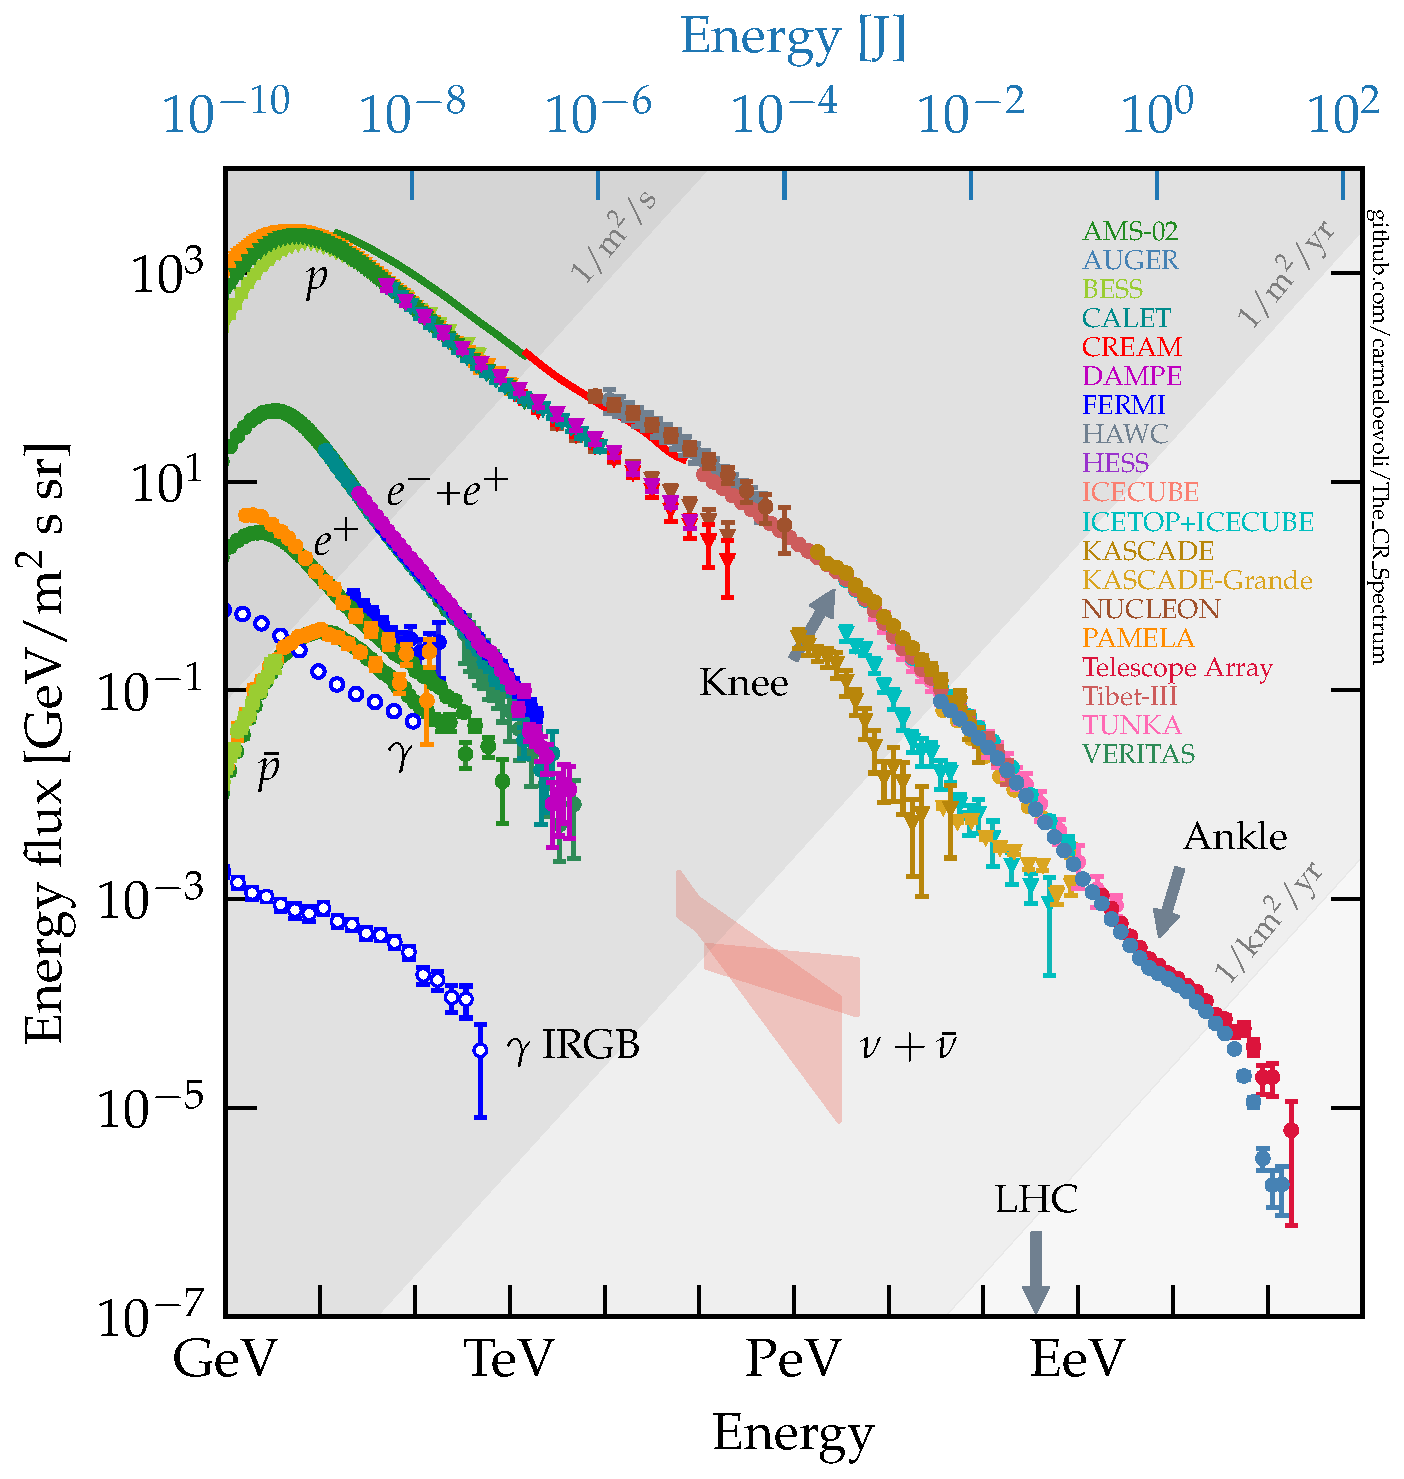
\includegraphics[width=0.46\textwidth]{graphics/cr_spectrum.pdf}
    \caption{The cosmic ray flux as a function of energy. For very high energies the flux becomes very
    small with only \(\num{1}\) particle per square meter per year reaching Earth. For even higher
    energies in the domain of \si{\exa\eV} this flux becomes \(\num{1}\) particle per square
    kilometer per year \cite{carmelo_2020}.}
    \label{fig:flux}
\end{wrapfigure}
where the gamma-ray flux is low, whereas lower energies show higher fluxes. Because the effective
collection area of space-based instruments such as \gls{fermilat} is too small \cite[p.~256]{funk},
they will see fewer high-energy events compared to ground-based experiments. The cosmic ray flux in
\autoref{fig:flux} shows this well: The flux decreases rapidly with higher energies, with only one
high-energy (\greater\(\SI{40}{\giga\eV}\)) photon per day and square meter reaching Earth from the Crab Nebula \cite{noethe_thesis}
and even fewer photons for energies in the \si{\exa\eV} domain, where only \(\num{1}\) particle per
square kilometer per year reaches Earth.

Earth's atmosphere is opaque to \gls{he} gamma rays, so ground-based experiments rely on
cascades of sub-particles in so-called \glspl{eas}. For gamma-ray astronomy, the electromagnetic
component of these \glspl{eas}, shown in \autoref{fig:heitler_model}, is of interest, as these
are produced by gamma rays. When a gamma ray interacts with Earth's atmosphere, it decays into an
electron and a positron via pair production. These charged particles then emit more photons via
bremsstrahlung. These photons, again, produce more charged particles, which in turn emit more
photons. This process continues until any of these processes reaches energies below a certain
threshold, \ie \SI{1022}{\kilo\eV} for the pair production process. For these processes to happen,
the particles have to be in the fields of the atoms of the Earth's atmosphere. As the particles
travel at speeds faster than light in the atmosphere, they emit Cherenkov light at
a fixed angle \(\theta\) with respect to the refraction index \(n\) of the atmosphere and the
factor \(\beta = \sfrac{v}{\symup{c}}\). The angle can be determined trigonometrically as
\begin{equation}
    \cos\theta = \frac{1}{\beta n},
\end{equation}
as can be seen in \autoref{fig:cherenkov}.

\begin{figure}
    \begin{subfigure}[t]{0.45\textwidth}
        \centering
        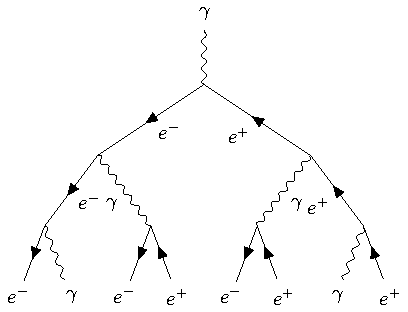
\includegraphics[width=0.90\textwidth]{graphics/heitler_model.pdf}
        \caption{Simplified first steps of the Heitler model of the electromagnetic component of an extensive air shower.
        A gamma ray induces an electron and a positron via pair production that then emit more photons
        via bremsstrahlung.}
        \label{fig:heitler_model}
    \end{subfigure}
    \hfill
    \begin{subfigure}[t]{0.45\textwidth}
        \centering
        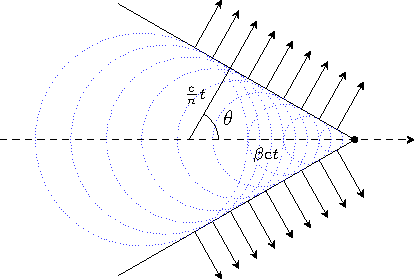
\includegraphics[width=0.90\textwidth]{graphics/cherenkov_radiation.pdf}
        \caption{Cherenkov radiation (outward-pointing arrows) from a charged particle traveling at
        uniform velocity, faster than the speed of light in the medium. The dashed line shows the
        path of the particle over time.}
        \label{fig:cherenkov}
    \end{subfigure}
    \caption{The electromagnetic component of an extensive air shower (see \hyperref[fig:heitler_model]{(a)})
    is induced by gamma rays that then decay into electrons and positrons via pair production.
    These charged particles will emit more gammas via bremsstrahlung, which again will produce
    new electrons and positrons. This will continue until \eg the energy of the gammas is below
    the threshold of \SI{1022}{\kilo\eV} for pair production. Another process is the production of
    Cherenkov light from the electrons and positrons, which is shown in \hyperref[fig:cherenkov]{(b)}.
    The Cherenkov light is the result of the charged particles traveling faster than the speed of light
    in the atmosphere, thus emitting photons in a fixed angle \(\theta\) \wrt the refraction index
    \(n\) of the medium and the factor \(\beta\).}
    \label{fig:cherenkov_heitler}
\end{figure}

Cherenkov light emitted by \glspl{eas} can then be collected by an IACT's mirrors and detected by
its camera within a timeframe of an order of nanoseconds. The resulting image will show the shape
of the air shower and can be used to determine the shower's primary particles' properties and
reconstruct its origin. As the hadronic component of \glspl{eas} produce
electromagnetic subshowers, \glspl{iact} have a dominant hadronic background, which has to be
separated from the gamma ray-induced showers, for example with
machine learning algorithms. This work, however, does not focus on these algorithms, but instead
on cleaning algorithms that are used to separate the signal from the electronic noise coming from the
camera as well as from the \gls{nsb}. This is a vital step in the analysis of an event, as only a
fraction of all pixels in the camera frame are part of the signal.


\section{The Cherenkov Telescope Array}
\label{sec:cta}

\cta{} is a new generation of \glspl{iact} that will consist of two sites,
one of which will be built at the \gls{orm} on the Canarian island of La Palma while the other
will be built in the southern hemisphere at the \glspl{eso} Paranal Observatory in the Atacama desert
of northern Chile. In this work, I will focus on the northern array, also called \cta{} north,
on La Palma.

\cta{} consists of three types of telescopes, shown in \autoref{fig:cta_telescopes}, each being
sensitive to a different energy range \cite{cta_specs}:
\begin{description}
    \item [] \textbf{\gls{lst}}: The largest telescopes in \cta{} have a primary deflector diameter
    of \SI{23}{\meter} with a field of view of \SI{4.3}{\deg} and provide full system sensitivity in the energy
    regime from \(\SI{20}{\giga\eV}\) to \(\SI{150}{\giga\eV}\).
    \item [] \textbf{\gls{mst}}: The \glspl{mst} have a primary deflector diameter of \SI{11.5}{\meter}
    with a field of view of \SI{7.7}{\deg} for their NectarCam and provide full system sensitivity in the energy
    regime from \(\SI{150}{\giga\eV}\) to \(\SI{5}{\tera\eV}\).
    \item [] \textbf{\gls{sst}}: Being the smallest telescope type in \cta{}, the \glspl{sst}
    have a primary deflector diameter of \SI{4.3}{\meter}, a secondary deflector diameter of
    \SI{1.8}{\meter} with a field of view of \SI{10.5}{\deg} and provide full system sensitivity in the energy
    regime from \(\SI{5}{\tera\eV}\) to \(\SI{300}{\tera\eV}\).
\end{description}

\begin{figure}
    \centering
    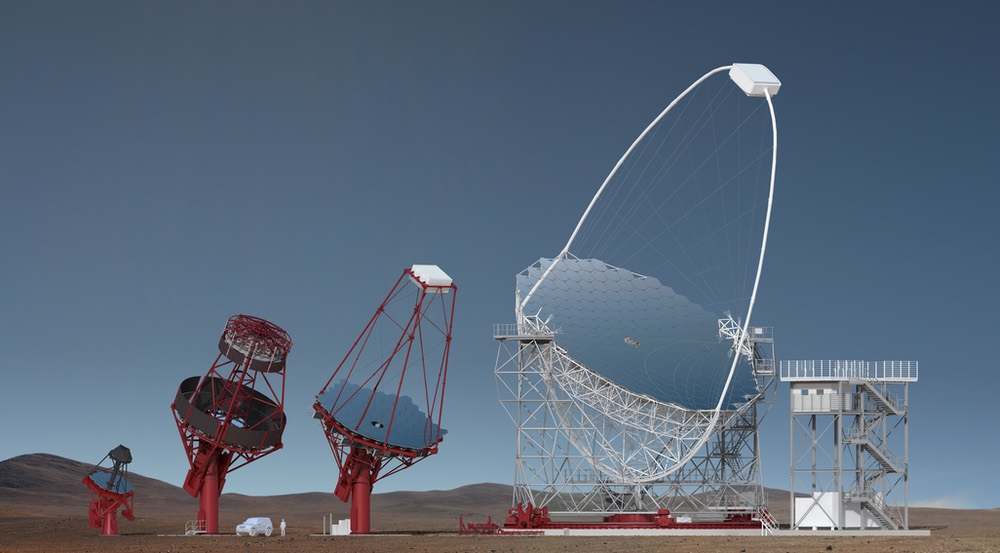
\includegraphics[width=0.7\textwidth]{graphics/telescopes_render.jpg}
    \caption{A rendered image of the 3 telescope prototypes in \cta{}. From left: The \gls{sst},
    two types of \gls{mst} (SCT and MST) and the \gls{lst}. This work will not feature the SCT, as
    the used simulation data contains only \gls{lst} and \gls{mst} data for the northern array.
    Image credit: Gabriel Pérez Diaz, IAC \cite{cta_tech}.}
    \label{fig:cta_telescopes}
\end{figure}

Since the southern hemisphere has a better view of the galactic center than the northern hemisphere,
only \cta{} south will feature the \glspl{sst} along the other two telescope types. \cta{} north
will only feature \glspl{mst} and \glspl{lst}. In its full configuration, \cta{} would feature
\(\num{70}\) \glspl{sst}, \(\num{25}\) \glspl{mst} and \(\num{4}\) \glspl{lst} at \cta{} south,
and \(\num{15}\) \glspl{mst} and \(\num{4}\) \glspl{lst} at \cta{} north. However, the reduced
layout---called Alpha Configuration---is the currently planned layout for both \cta{}
north and south. This work will focus on the northern site, consisting of \(\num{9}\) \glspl{mst}
and \(\num{4}\) \glspl{lst} \cite{cta_north_layout}. \autoref{fig:cta_layout} shows the planned
Alpha Configuration layout of both sites of \cta{} where \cta{} south is displayed with its
\(\num{37}\) \glspl{sst}, \(\num{14}\) \glspl{mst} and the \(\num{4}\) \glspl{lst} in the center
\cite{cta_south_layout}.
\begin{figure}
    \centering
    % \includegraphics[width=0.75\textwidth]{graphics/cta_alpha_layout.pdf}
    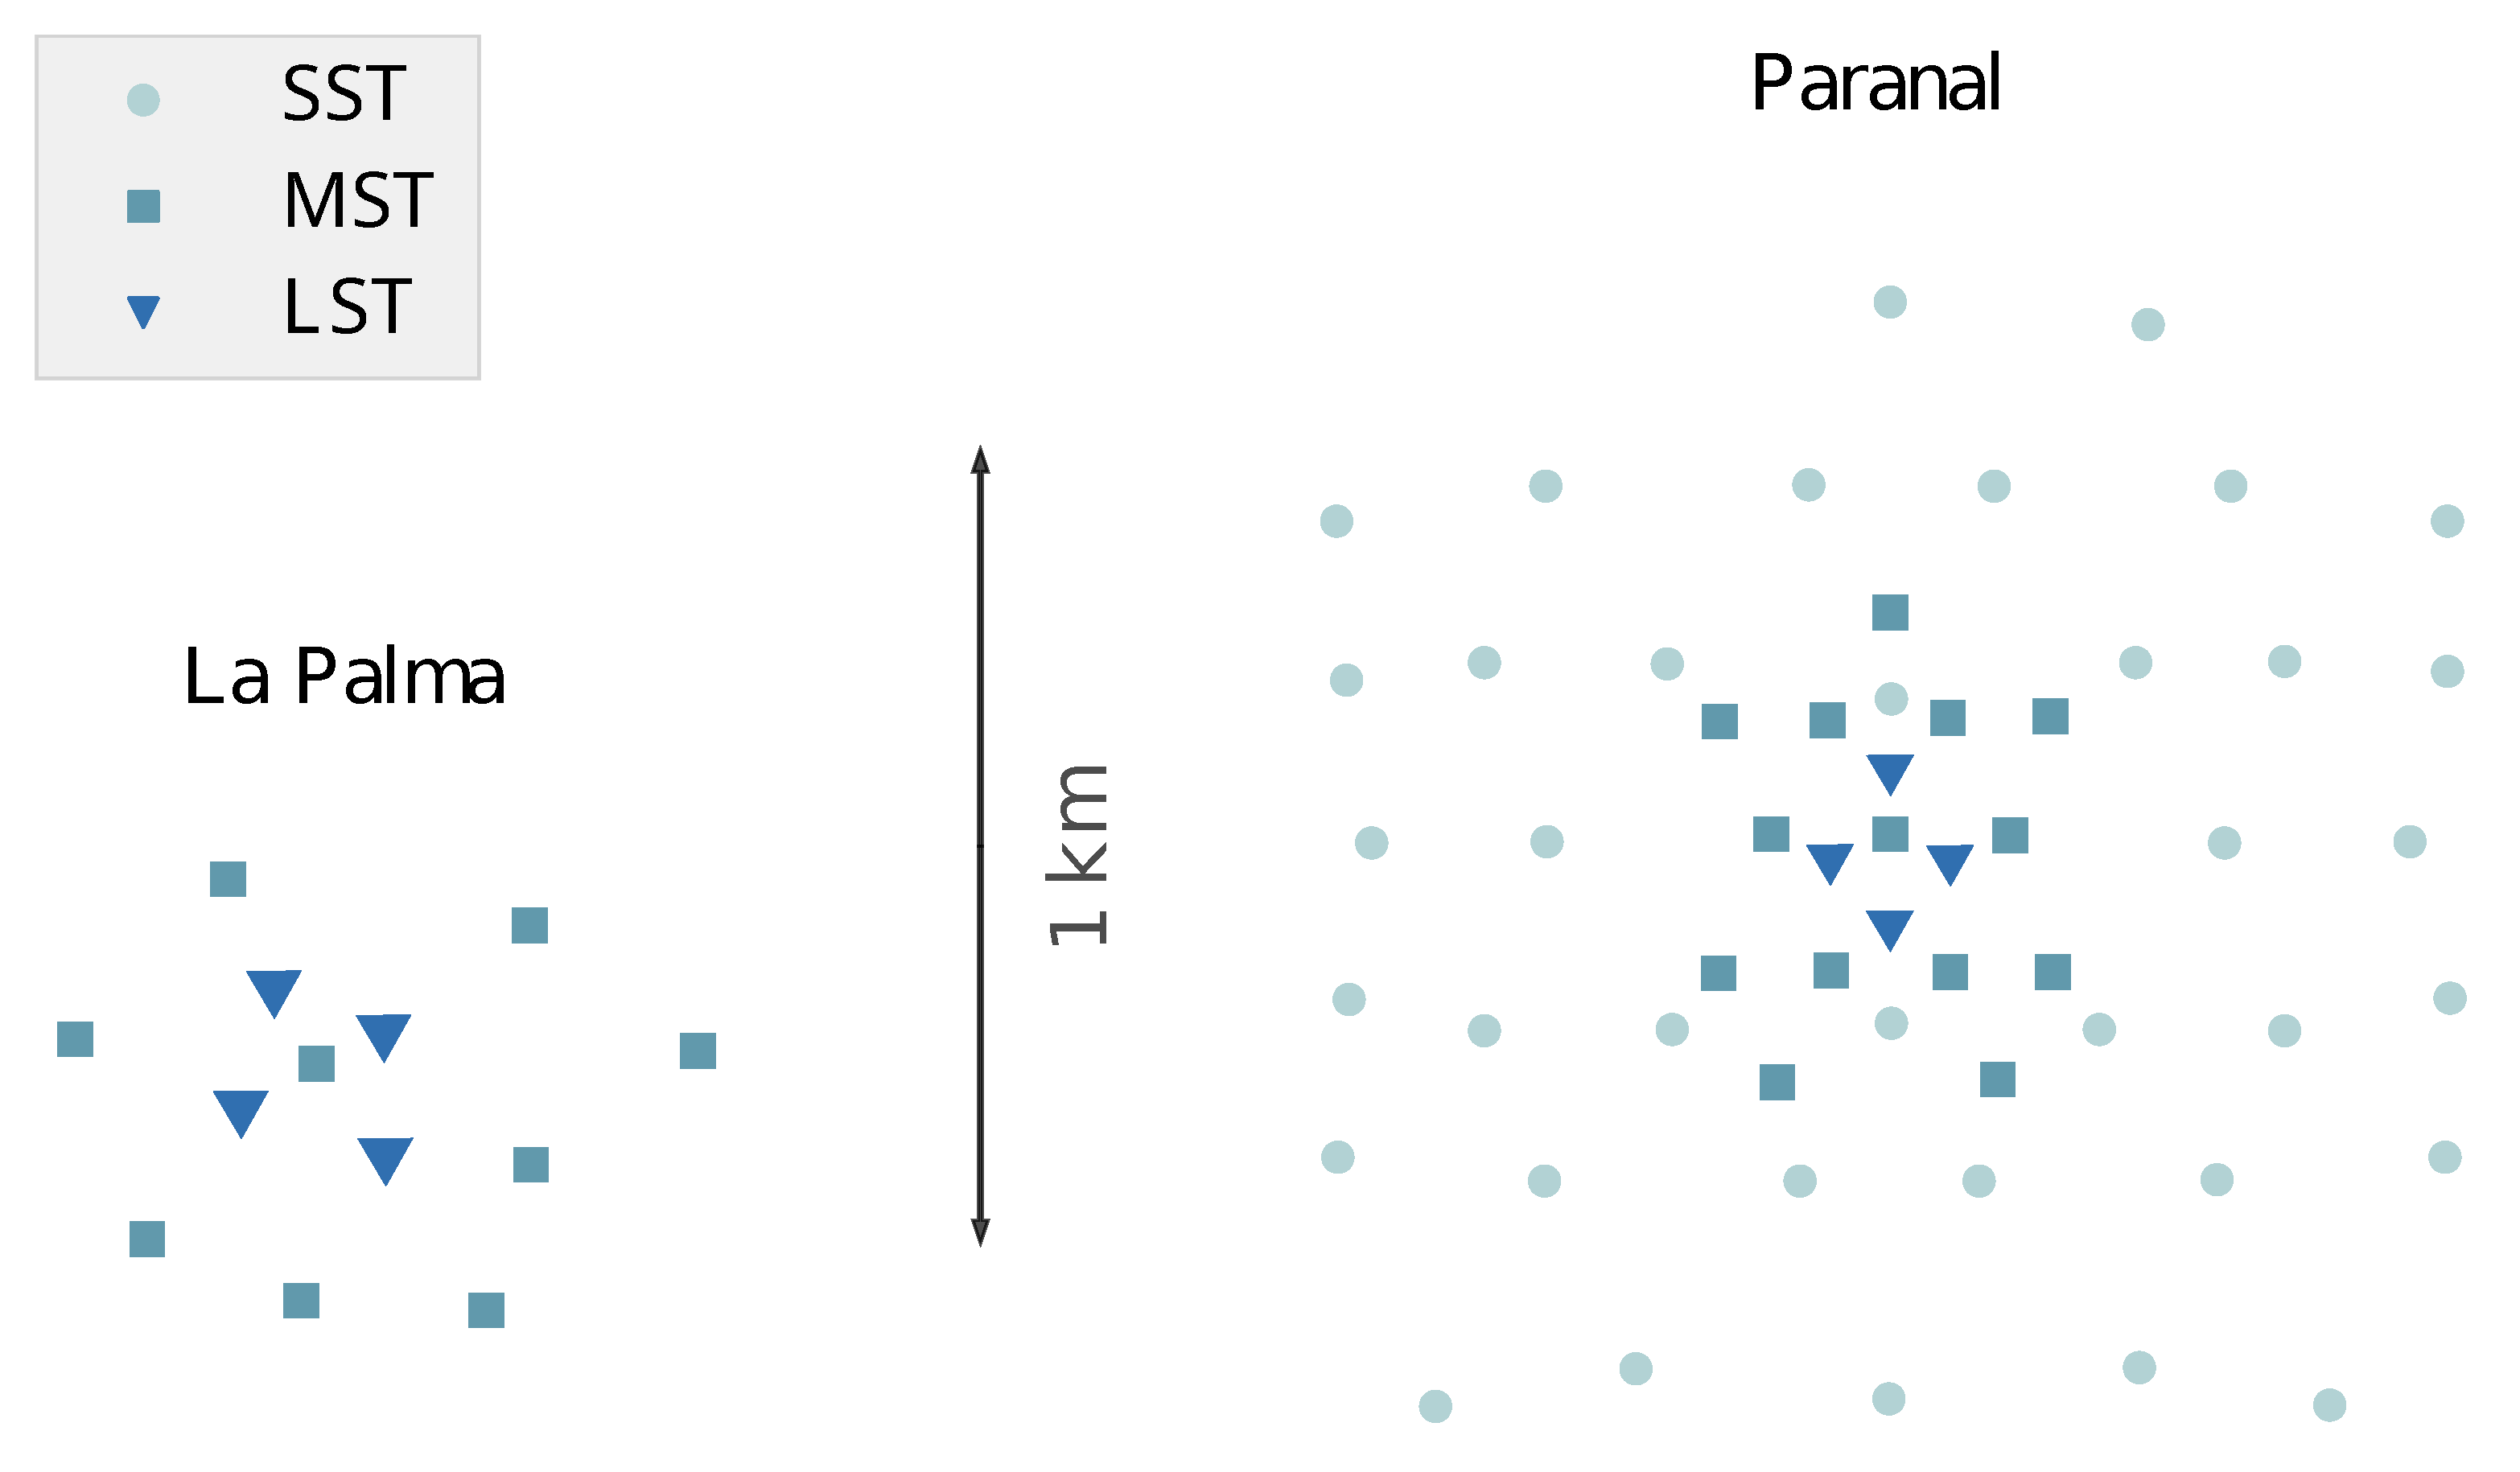
\includegraphics[width=0.75\textwidth]{graphics/cta_layout.pdf}
    \caption{Alpha Configuration layout of the \cta{} north and \cta{}
    south site. \cta{} south would feature \(\num{37}\) \glspl{sst}, \(\num{14}\) \glspl{mst} and
    \(\num{4}\) \glspl{lst} \cite{cta_south_layout} in it's Alpha Configuration, while \cta{} north would
    feature \(\num{9}\) \glspl{mst} and \(\num{4}\) \glspl{lst} \cite{cta_north_layout}.
    This figure was adapted from Kai Br\"ugge in his Ph.D. thesis \cite{bruegge_thesis}.}
    \label{fig:cta_layout}
\end{figure}

The \gls{mst}'s and \gls{lst}'s cameras are based on \gls{pmt} photodetectors, while the \gls{sst}'s
camera is based on a \gls{sipm} photodetector. Both detector types provide fast response times in the
order of nanoseconds. \glspl{pmt} can detect small amounts of electromagnetic radiation due to their
amplification process. However, this amplification process also amplifies the noise of the detector
and also needs higher voltages than \glspl{sipm}. The latter, on the other hand, needs to be cooled,
as \glspl{sipm} are prone to have a higher dark current at higher temperatures.
% The \gls{mst} and \gls{lst} will feature a camera with \(\num{1855}\) pixels.

With \cta{} probing the \gls{vhe} gamma-ray sky and a resolution outperforming predecessors, like
\gls{hess} or \gls{magic}, it will be able to observe a broad variety of sources, allowing insights
into interaction processes of \gls{vhegr} as well as their origin.

Together with gravitational wave and neutrino observatories as well as with other photon observatories,
\cta{} will probe the universe in its \glsreset{he}\gls{he} domain, allowing to study a broad field of key questions
in astrophysics. As such, \cta's scientific goals can be divided into three categories \cite{cta_scientific_goals}:
\begin{description}
    \item [Origin and Role of relativistic Cosmic Particles:] \cta{} will try to find the sources of
    \gls{he} cosmic particle acceleration in the universe. This includes the search for the mechanisms
    that accelerate cosmic particles. Also, \cta{} will try to answer what role these particles play
    in feedback on star formation and galaxy evolution.
    \item [Extreme Environments:] \cta{} aims to deepen our understanding of the processes that
    are at work close to neutron stars and black holes, the characteristics of relativistic jets and
    \gls{pwn}. Also, it will probe how intense radiation fields and magnetic fields are and how these
    would evolve over cosmic time scales.
    \item [Frontiers in Physics:] \cta{} will try to answer questions about the nature of dark matter
    and its distribution in the universe. As such, the existence of axion-like particles will be
    probed. Furthermore, \cta{} will search for quantum gravitational effects on photon propagation.
\end{description}

